\documentclass{beamer}
\usetheme{Dresden}
\usepackage[utf8]{inputenc}

\title{Abschlusspräsentation}
\author{Team ILIAS}
\date{\today}

\begin{document}
	\maketitle
	\frame{\tableofcontents[]}
	\section{Teamaufteilung}
	\begin{frame}
		\frametitle{Aufteilung des Teams}
		\begin{center}
			\begin{tabular}{|c|c|}\hline
				Teammitglied & Aufgabe \\\hline
				Josephine Rehak & Chefprogrammiererin\\\hline
				Richard Mörbitz & Assistent\\\hline
				Max Friedrich & Administrator\\\hline
				Peter Merseburger & Testverantwortlicher\\\hline
				Julius Felchow & Sekretär\\\hline
			\end{tabular}
		\end{center}
	\end{frame} 
 
	\section{Aufgabe}
		\begin{frame}
			\frametitle{Einführung zur Thematik}
			ILIAS:
			\begin{itemize}
  				\item E-Learning Plattform
  			 	\item Erstellung von Frage für Klausuren
  				\pause
  				\\
    			\item nicht vorhanden: Reviews
    		\end{itemize}
		\end{frame}
		\begin{frame}
			\frametitle{Einführung zur Thematik}
			Reviews:
			\begin{itemize}
				\item Bewertung einer Frage
				\item durch fremde Person
				\item nach Vorgabe von Prof. Wollersheim
			\end{itemize}
		\end{frame}
		\begin{frame}
			\frametitle{Aufgabenstellung}
			\begin{itemize}
				\item ILIAS-Fragen für Reviews nutzbar machen
				\pause
				\item Erstellen von Reviews zu ILIAS-Fragen
				\pause
				\item Händische Zuordnung von Reviewern zu Fragen
				\pause
				\item Übersicht über eigene erstellte Fragen und Reviews
			\end{itemize}
		\end{frame}
		\begin{frame}
			\begin{center}
				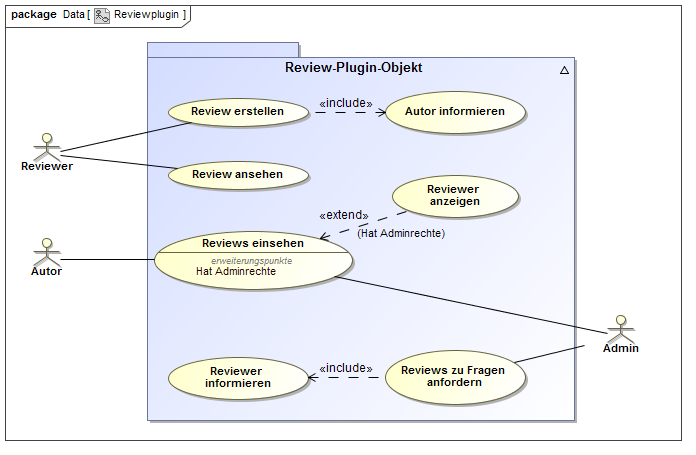
\includegraphics[scale=0.45]{Diagramme/Use_Case_Diagram__Reviewplugin.png}
				\label{Reviewplugin}
			\end{center}
		\end{frame}
		\begin{frame}
			\begin{center}
				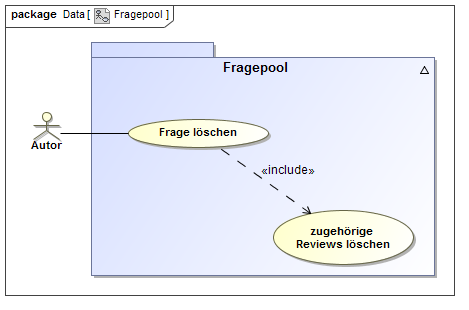
\includegraphics[scale=0.5]{Diagramme/Use_Case_Diagram__Fragepool.png}
				\label{Fragepool}
			\end{center}
		\end{frame}
	\section{Probleme}
		\begin{frame}
			\frametitle{Probleme}
    		\begin{itemize}
		    	\item Definition der reviewbaren Fragen
		    	\pause
    			\item Wahl der Reviewer-Zuordnung
    			\pause
    			\item Erstellung und Durchführung der Tests
    			\pause
    			\item Erfüllung der Wunschkriterien
    		\end{itemize}
		\end{frame}
	\section{Umsetzung}
		\begin{frame}
			\frametitle{Erfüllung der Musskriterien}
			\begin{itemize}
				\item Review-Maske gemäß Prof. Wollersheims Beispiel
				\pause
				\item Expertise nach Frau Kombrinks Wunsch
				\pause
				\item Einordnung in Wissensdimension und Taxonomie durch Autor und Reviewer
				\pause
				\item "Ghost-Reviewing"
				\pause
				\item Reviewbarer Fragetyp (Multiple Choice)
			\end{itemize}
		\end{frame}
		\begin{frame}
			\begin{center}
				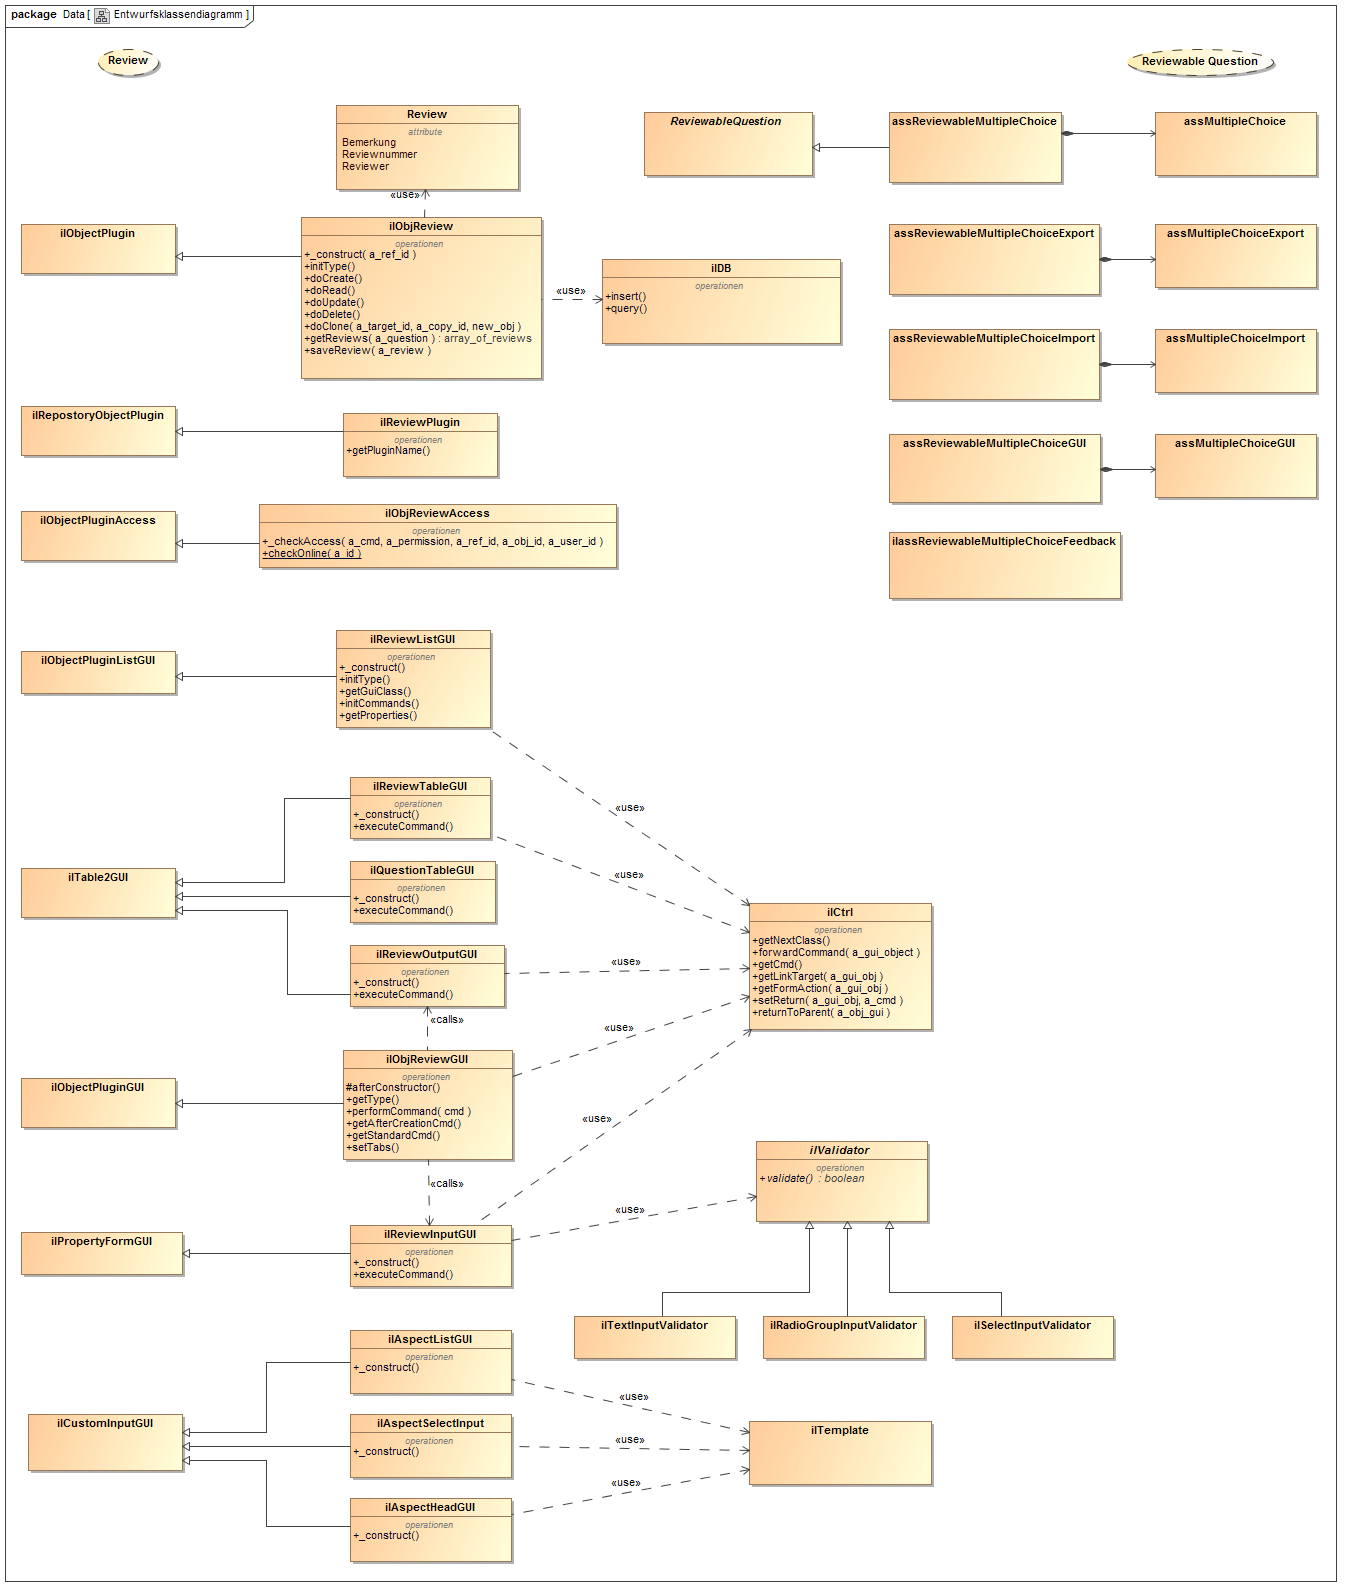
\includegraphics[scale=0.08]{Diagramme/Class_Diagram__Entwurfsklassendiagramm.png}
			\end{center}
		\end{frame}
		\begin{frame}
			\begin{center}
				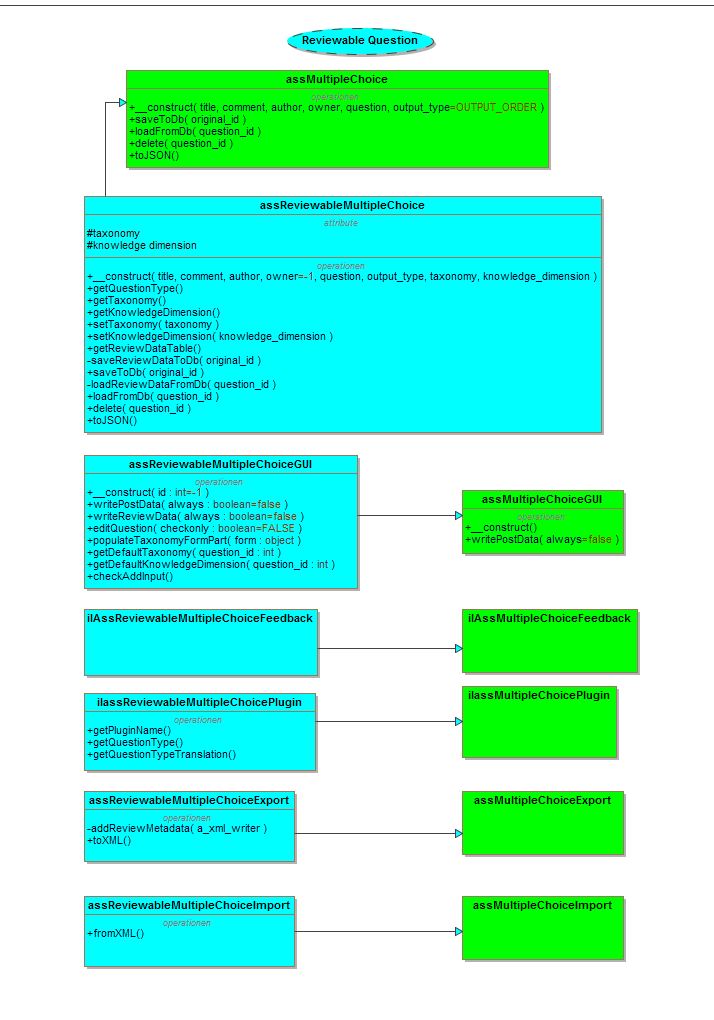
\includegraphics[scale=0.20]{Diagramme/Class_Diagram__Entwurfsklassendiagramm(2).png}
				\label{Reviewplugin}
			\end{center}
		\end{frame}
		\begin{frame}
			\begin{center}
				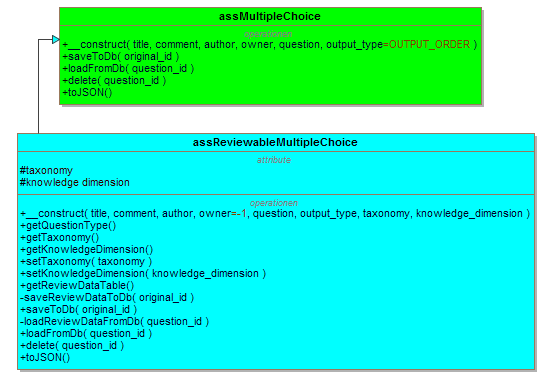
\includegraphics[scale=0.45]{Diagramme/Class_Diagram__Entwurfsklassendiagramm(3).png}
			\end{center}
		\end{frame}
		\begin{frame}
			\begin{center}
				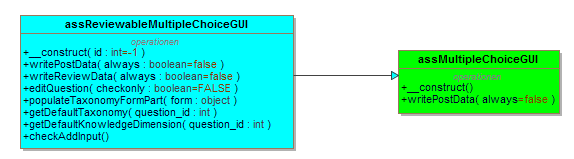
\includegraphics[scale=0.45]{Diagramme/Class_Diagram__Entwurfsklassendiagramm(4).png}
			\end{center}
		\end{frame}
		\begin{frame}
			\begin{center}
				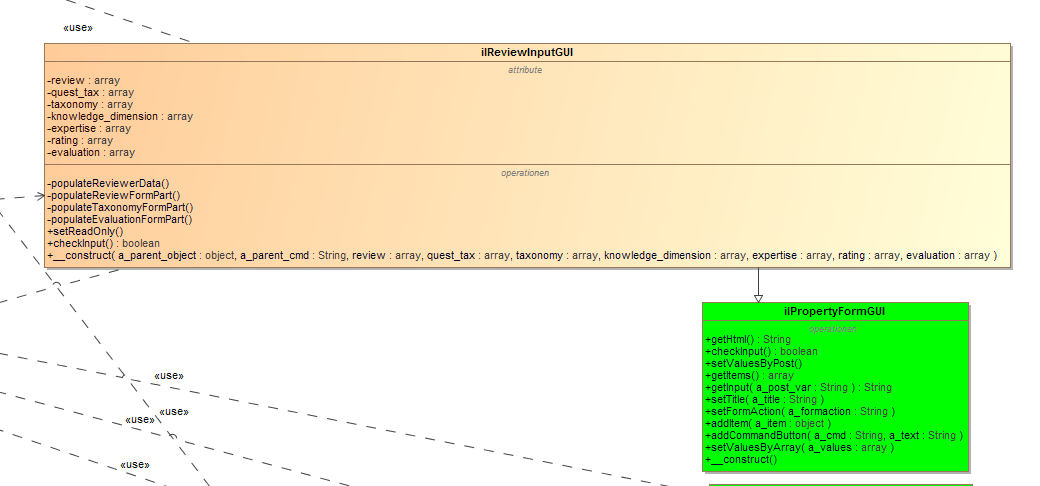
\includegraphics[scale=0.3]{Diagramme/Class_Diagram__Entwurfsklassendiagramm(5).png}
			\end{center}
		\end{frame}
		\begin{frame}
			\begin{center}
				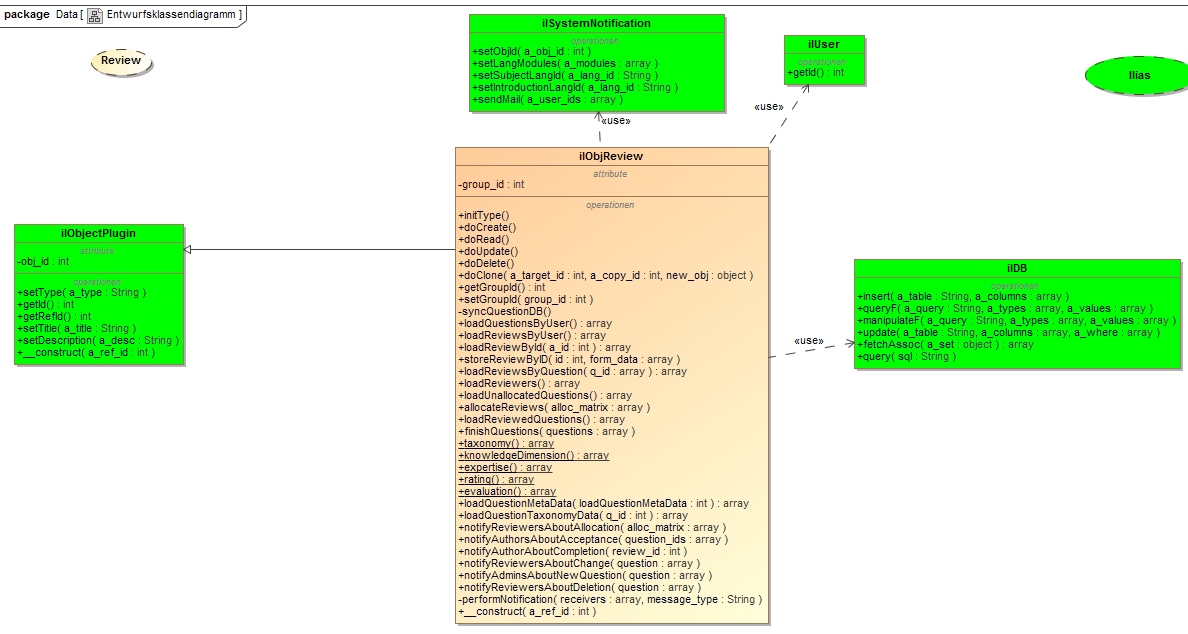
\includegraphics[scale=0.25]{Diagramme/Class_Diagram__Entwurfsklassendiagramm(6).png}
			\end{center}
		\end{frame}
		\begin{frame}
			\begin{center}
				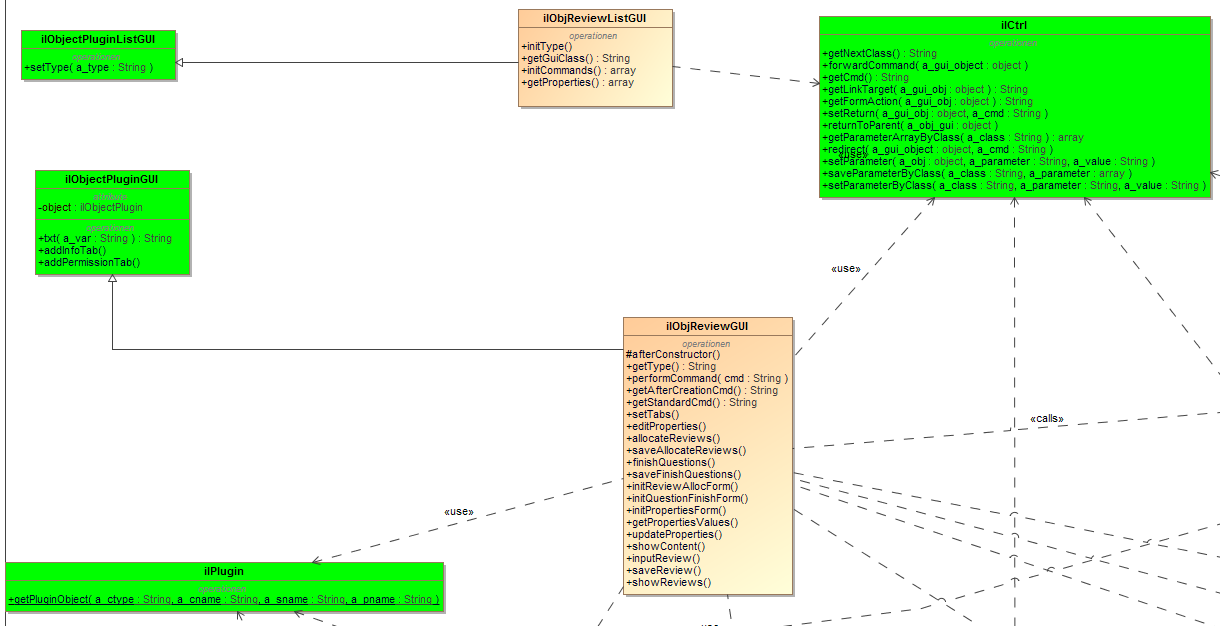
\includegraphics[scale=0.25]{Diagramme/Class_Diagram__Entwurfsklassendiagramm(8).png}
			\end{center}
		\end{frame}
	\section{Vorstellung des Resultats}
		\begin{frame}
			\begin{center}
				Live-Demo
			\end{center}
		\end{frame}
\end{document}